\section{rSLA deployment }

rSLA Service has literally been evolved on the IBM Bluemix PaaS as a ruby Sinatra application. As shown in Figure~\ref{fig:runtime}, the different components involved in SLA 
management are deployed in Bluemix. The following section will explain further how rSLA interoperates with the other services (Scheduler, Cloudant, Xlets) in a real use case. 

\begin{figure}[H]
\centering
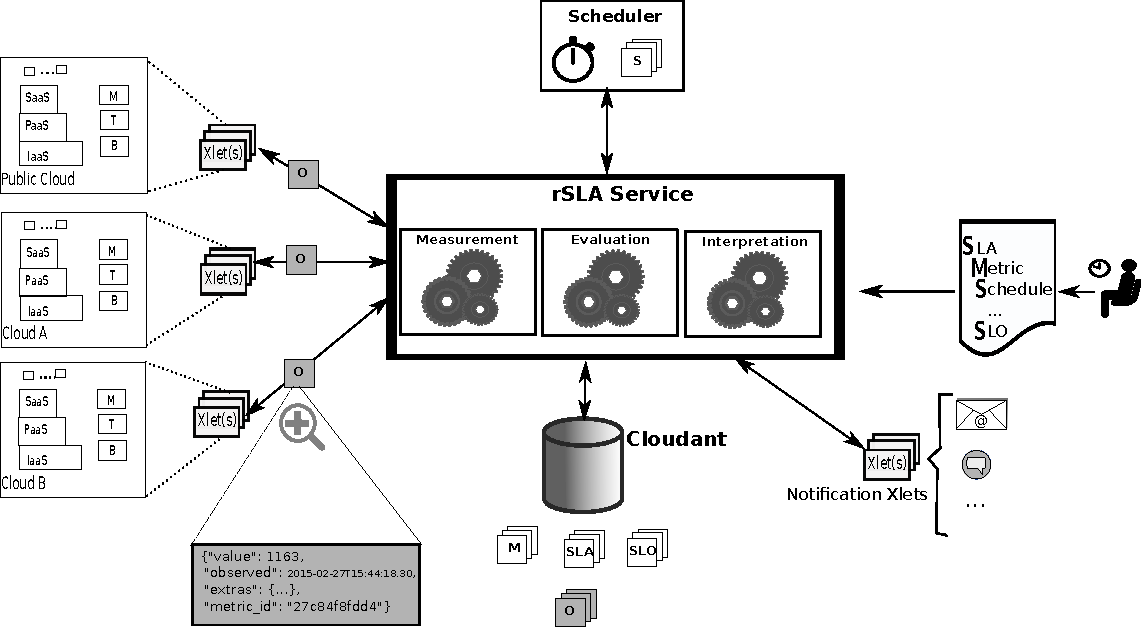
\includegraphics[width=\textwidth]{pics/runtime.pdf}
\caption{\label{fig:runtime} rSLA runtime}
\end{figure}


\subsection{Ameriprise pilot}

Currently, the rSLA service supports the management of cloud services that are leased by an existing customer. In one agreement, the IBM customer migrated a workload from a customer-owned, on-premise data center environment to the IBM cloud.  Along with the move, the customer required the monitoring of seven custom SLAs that had never been offered previously by the service provider in the cloud.

Each of the seven running SLAs consist of one base metric and one service level objective. The rSLA service that is running on the Bluemix platform, is aware of these seven agreements' context as such information is parsed by the rSLA engine to activate and initiate the measurement of involved base metrics. The rSLA service monitors, measures, evaluates and reports the service level status of the seven involved SLOs on a daily basis to the customer. 

%can we add a graph showing statistics on the rSLA service usage/performance since we started the ameriprise pilot? Bluemix?
%or from cloudant?



\subsection{rSLA service}
rSLA Service is a Sinatra application deployed on Bluemix PaaS. It offers different REST interfaces that allow the management of the life cycle of an SLA described using our DSL.
At the reception of a new SLA, rSLA Service interprets the file and creates ruby objects based on the DSL. The new objects are persisted in Cloudant using CouchRest Model.
On the activation of an SLA, rSLA Service orchestrates all the needed operations to activate and manage the SLA life cycle. It starts by scheduling data collection for base 
metrics. As shown in Figure~\ref{fig:runtime}, based on the defined schedules, the scheduler triggers the needed rSLA Service interfaces. This latter will then invoke the 
Monitoring Xlets to collect new observations for the related base metrics. Afterwards, the observations are persisted in Cloudant. Similarly, on the schedule of an SLO, the 
Scheduler triggers a rSLA Service interface for SLO evaluation. rSLA will then evaluate the data related to the specific SLO. This evaluation implies 
eventually the usage of map-reduce functions offered by Cloudant. We made this decision in order to delegate all the possible parallel processings to Cloudant and benefit from its 
efficiency. Afterwards, rSLA Service generates JSON notifications representing the results of the evaluation. These notifications are sent to the Notification Xlet for 
formatting and reporting to the client.   
\subsection{rSLA Xlets}
During its life-cycle, rSLA Service requires different services to ensure the management of SLAs. These services are eventually offered as services through Bluemix PaaS. At the 
time being, rSLA uses one offered service for persistence and a list of services for monitoring and reporting. These latter, are provided as Xlets. An Xlet is a light weight 
application offered as a service through Bluemix PaaS. This application is designed to facilitate the integration of different offered services spanning over the different layers 
of the Cloud by providing a generic REST API. An Xlet is customized according to its role in the overall system. As shown in Figure~\ref{fig:xlet}, each Xlet provides three 
interfaces:
\begin{itemize}
 \item \emph{CFBrokerInterface}: Since the Xlets are provided as services by Bluemix PaaS, they need to offer this generic interface that describes exactly how to provision the 
service, how to unprovision it, how to bind the service to a given application and how to unbind it. 
\item  \emph{ConfigurationInterface}: In order to ensure multi-tenancy and customization of an Xlet, it should offer an interface to configure its tenancy. This interface could 
offer other functionalities of customization. It allows in some cases to configure the access credentials for Cloud resources.
\item  \emph{RuntimeInterface}: This interface describes the main business of the Xlet. It describes the specific functionalities to be offered by the application instance (e.g., 
monitoring services, reporting services). 
\end{itemize}
\begin{figure}[H]
\centering
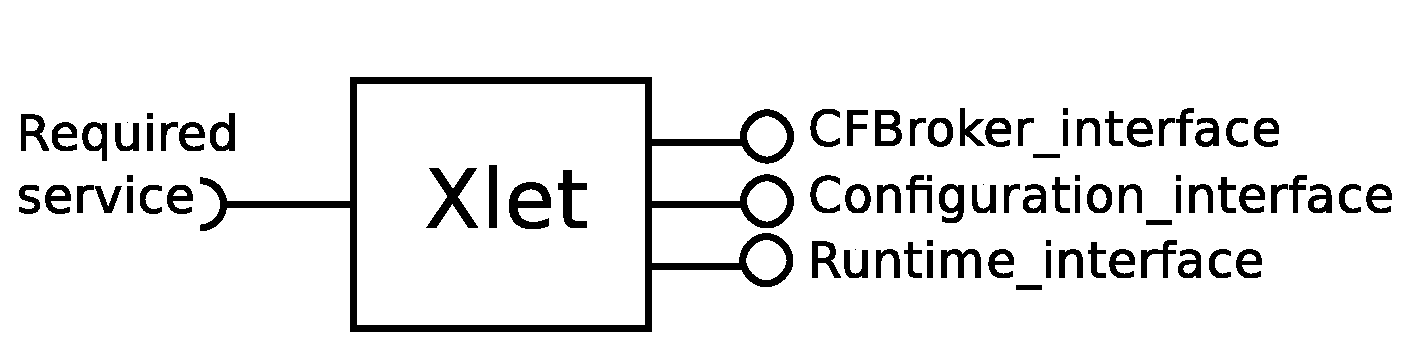
\includegraphics[width=0.6\textwidth]{pics/Xlet}
\caption{\label{fig:xlet} Xlet generic design}
\end{figure}

All Xlets respect the same architecture but differs in their implementations from a use case to another. In our current work we defined different monitoring and reporting Xlets. 
Monitoring Xlets are in-line with the DMTF standard. They allow collecting monitoring data for a specific type of resources with different granularities. For example, 
Figure~\ref{fig:slxlet} shows a SoftLayer specific Xlet. SLXlet allow to get monitoring data of SoftLayer provisioned servers for a given account. The account credentials are 
passed to the Xlet in the configuration phase through the Configuration interface. Afterwards, the Runtime interface of the Xlet could be used to get the list of servers, the list 
of metrics for a given server or, the value for a given metric for a specific server.

\begin{figure}[H]
\centering
\hspace{1.5cm}
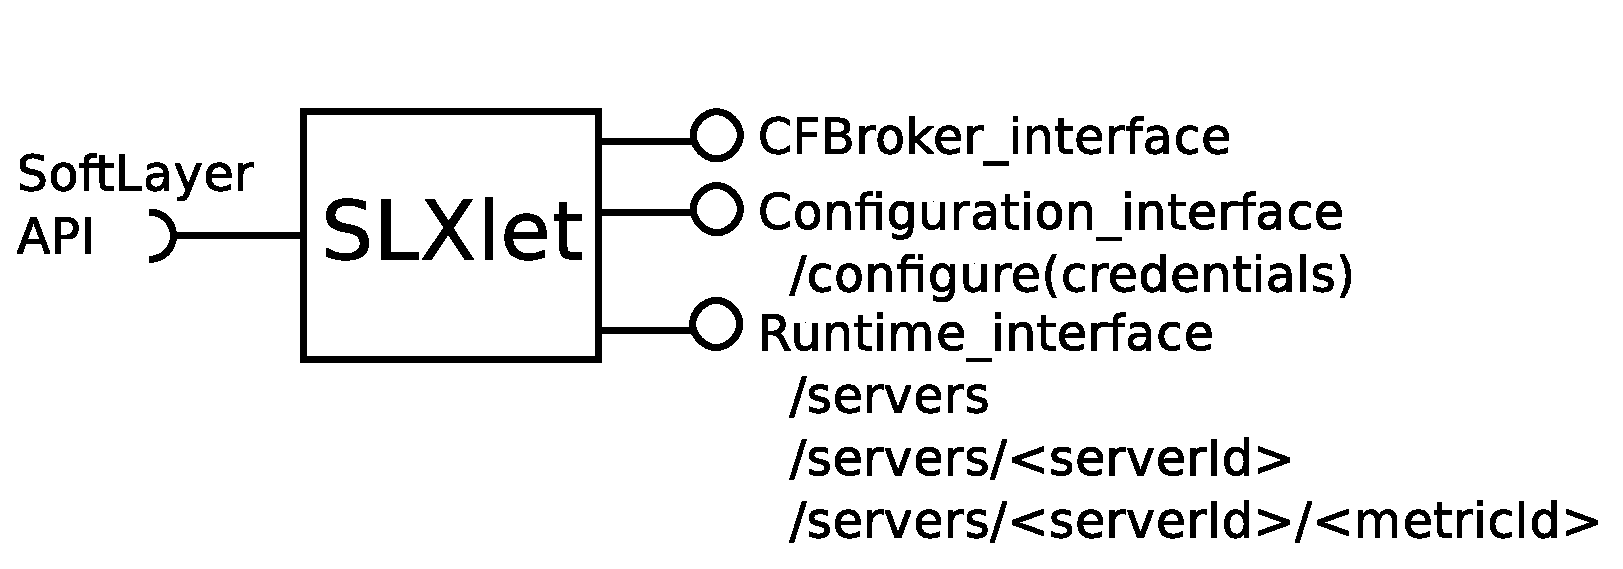
\includegraphics[width=0.7\textwidth]{pics/SLXlet}
\caption{\label{fig:slxlet} SoftLayer Xlet design}
\end{figure}

Using Xlets within Bluemix PaaS has been very helpful. The advantageous characteristics of using Xlets in this environment are the following:
\begin{itemize}
 \item Scalability: this characteristic is inherited from the scalability of Bluemix environment. Since the Xlet could be provisioned as an application or a service within 
Bluemix, it is easy to scale it horizontally to cope with the work load by adding or removing new instances,
\item Reusability: all Xlets have a common and generic core code that allow the easy reusability with minor modifications for specific use case, 
\item Manageability: managing Xlets is handled to Bluemix, the management here includes provisioning, deprovisioning, binding and unbinding Xlets to other applications,
\item Flexibility: Xlets could be integrated easily using Bluemix services, they could be provisioned using different plans (e.g., shared or dedicated). 
\end{itemize}